\vspace{-2mm}
\section{Experiments}
\label{sec:experiments}

\begin{figure*}[!t]
    \centering
    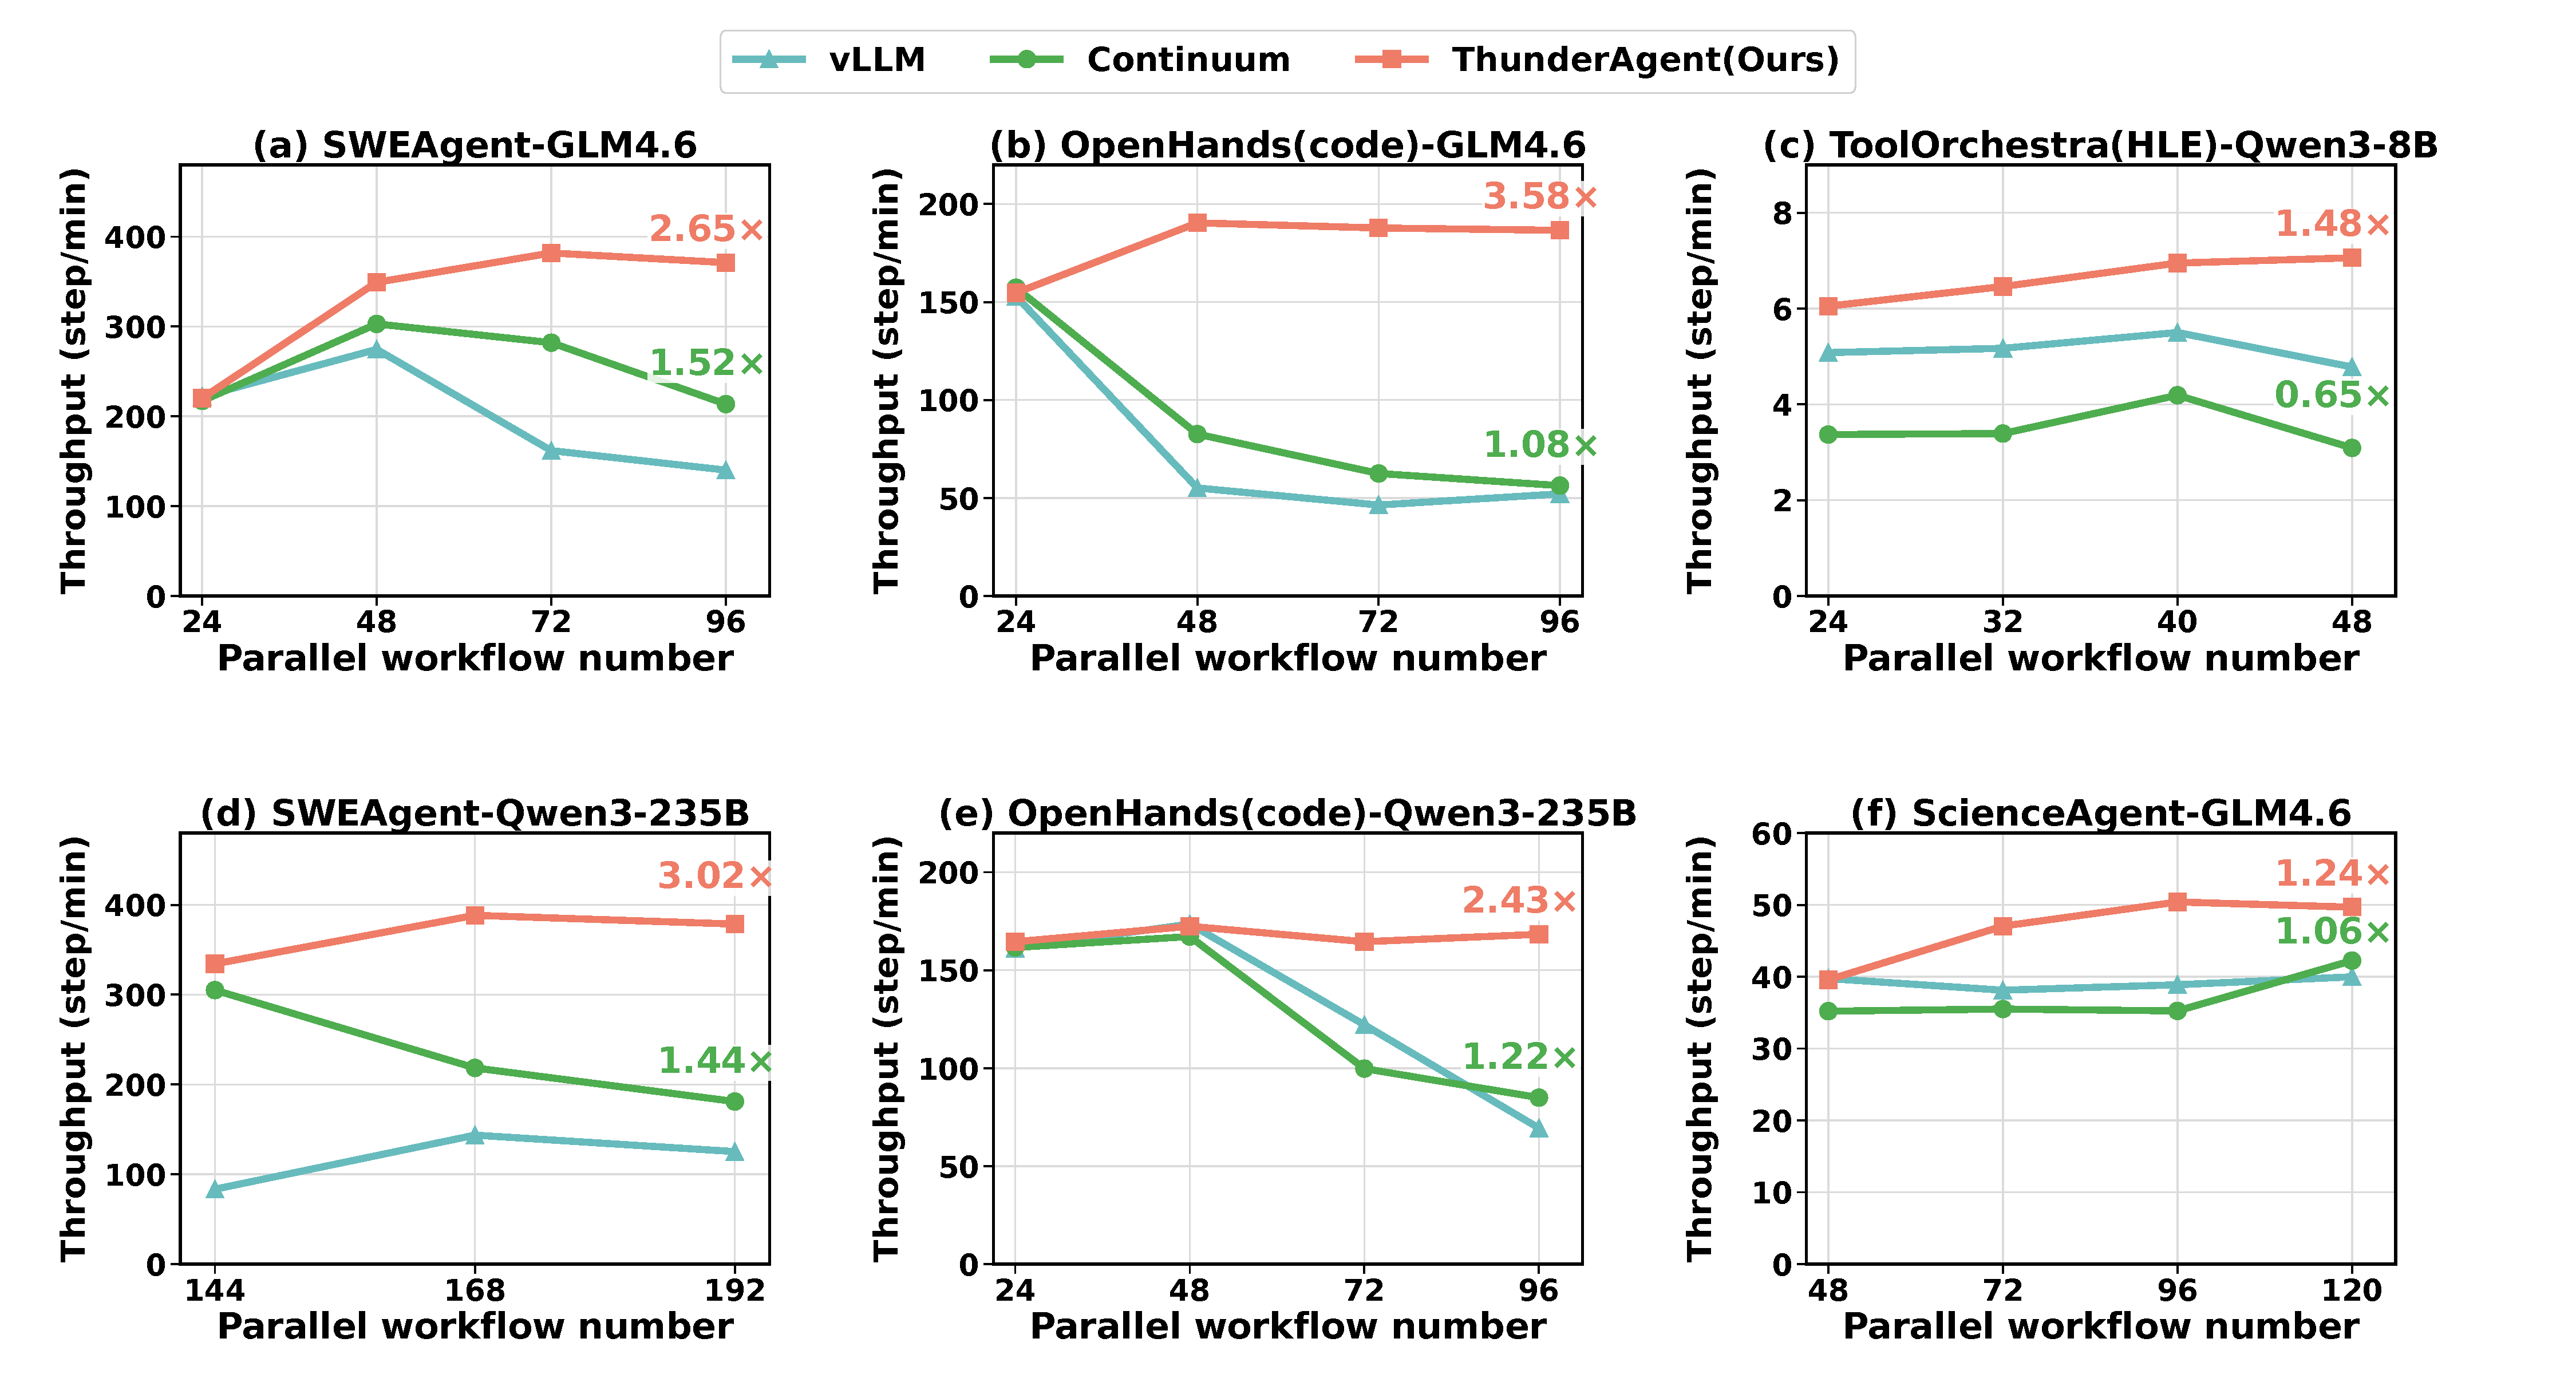
\includegraphics[width=1.0\columnwidth]{Figures/infer_eval.pdf}
    \caption{\textbf{Serving Evaluation Results.} \ouralg significantly outperforms vLLM and Continuum across three models, four agentic workflows, and three datasets. For workflows with predictable tool call times (e.g., a, b, d, e), \ouralg outperforms vLLM and Continuum up to 2.43-3.56$\times$. For workflows exhibit stochastic tool execution time (e.g., c, f), \ouralg still achieves the best throughput performance.}
    \label{fig:eval_infer_result}
    \vspace{-4mm}
\end{figure*}

In this section, we evaluate \ouralg on diverse agentic workflows, including coding, routing, and scientific research agents, and RL rollout across multiple hardware configurations ranging from RTX5090 to H100 clusters. Furthermore, we conduct extensive ablation studies to breakdown the end-to-end system runtime and to describe the system's sensitivity to the scheduler's hyperparameters, $\Delta t$ and $f(t)$, in \autoref{app:ablation_study}.
\vspace{-6mm}
\subsection{Experimental setup}
\label{sec:experiments setup}
\paragraph{Benchmarks and workflows.} We evaluate \ouralg against diverse benchmarks and workloads:
\begin{enumerate}[itemsep=0.0pt,topsep=2pt,leftmargin=*]
    % Item 1
    \item \textbf{Coding agent serving.} We deploy \textbf{OpenHands} and \textbf{mini-SWEAgent} on the SWEBench-Lite~\citep{jimenez2024swebenchlanguagemodelsresolve} dataset. OpenHands represents a \textbf{heavy-initialization workflow} with an average disk footprint exceeding 10GB per sandbox, while mini-SWEAgent is a \textbf{lightweight workflow} with a minimal footprint ($\approx$2GB).

    % Item 2
    \item \textbf{Other agent serving.} We apply ToolOrchestra on HLE~\citep{phan2025humanitysexam} and OpenHands on ScienceAgentBench~\citep{chen2024scienceagentbenchrigorousassessmentlanguage}. These workloads involve variable latencies driven by external API calls and complex scientific simulations.
    \item \textbf{RL rollout.} We apply the same models, workflows, and samples for RL rollout on two 8$\times$ H100 nodes.
\end{enumerate}
\paragraph{Models and deployments.}
% For OpenHands~\citep{wang2025openhandsopenplatformai} evaluated in science, code, and mini-SWEAgent~\citep{yang2024sweagentagentcomputerinterfacesenable}, we employ GLM-4.6 (355B)~\citep{5team2025glm45agenticreasoningcoding} and Qwen-3 (235B)~\citep{yang2025qwen3technicalreport}, which are optimized for complex agentic tasks. To further reduce the memory footprint, we compress these models to FP8. We apply Tensor Parallelism (TP=8) on single 8$\times$H100 nodes for serving tests. We deploy a Qwen3-8B model on a single RTX 4090 for ToolOrchestra~\citep{su2025toolorchestraelevatingintelligenceefficient} in FP16.
\vspace{-2mm}
We employ GLM-4.6 (355B) \citep{5team2025glm45agenticreasoningcoding} and Qwen-3 (235B)~\citep{yang2025qwen3technicalreport} using both OpenHands~\citep{wang2025openhandsopenplatformai} and mini-SWEAgent~\citep{yang2024sweagentagentcomputerinterfacesenable} frameworks. Models are quantized to FP8 with Tensor Parallelism (TP8) on 8$\times$H100 nodes. For ToolOrchestra~\citep{su2025toolorchestraelevatingintelligenceefficient}, we use Qwen3-8B with FP16 precision hosted on one RTX 5090. We deploy the LLM inference engine and Docker at different clusters. The LLM inference engine runs on GPU clusters hosting the models, while agent Docker environments are offloaded to a dedicated CPU cluster.

% \vspace{-1mm}
% \textbf{Benchmarks and workflows.} We gather a diverse set of benchmarks to evaluate \ouralg against workloads with distinct characteristics:

% \vspace{-1mm}
% \noindent\textit{(1) Coding Agents.} We deploy \textbf{OpenHands} and \textbf{mini-SWEAgent} on SWEBench-Lite~\citep{jimenez2024swebenchlanguagemodelsresolve}. OpenHands represents a \textbf{\textit{heavy-initialization} workflow}, requiring extensive Docker setup and unique dependency installation, with an average disk footprint exceeding 10GB per sandbox. In contrast, mini-SWEAgent represents a \textbf{\textit{lightweight} workflow} with a minimal footprint ($\approx$2GB).

% \vspace{-1.8mm}
% \noindent\textit{(2) Routing and Scientific Agents.}
% To assess resilience to \textbf{non-deterministic acting time}, we utilize ToolOrchestra on HLE dataset~\citep{phan2025humanitysexam} and OpenHands on ScienceAgentBench~\citep{chen2024scienceagentbenchrigorousassessmentlanguage}, which involve variable latencies from external API calls and scientific simulations. % due to remote model calling, web searches, and scientific simulations.
\vspace{-2mm}
\paragraph{\ouralg configuration.} We configure \ouralg with hyperparameters $\Delta t = 5$ and priority decay $f(t) = 2^{-t}$, defined in \autoref{sec:scheduling_policy}. vLLM is employed as our LLM inference engine. We use steps per minute as our throughput metric, where one step includes a reasoning and acting period of the workflow.
\vspace{-2mm}
\paragraph{Baseline techniques.}
We compare against state-of-the-art systems with different scheduling paradigms:

% \begin{itemize}
%     \item \textbf{vLLM (Inference):} A widely-adopted, request-aware inference engine. It serves as the baseline for standard serving performance without agent-specific awareness.
%     \item \textbf{Continuum (Inference):} The current state-of-the-art system for multi-turn agentic workflows. It mitigates thrashing by predicting tool execution durations and pinning KV caches to HBM accordingly.
%     \item \textbf{vLLM + SGLang Gateway (Distributed Rollout):} The leading solution for large-scale RL rollout. SGLang Gateway optimizes distributed inference by enhancing cross-node memory balancing and KV cache hit rates, making it a strong baseline for the rollout setting.
% \end{itemize}

\begin{itemize}[itemsep=0.0pt,topsep=0pt,leftmargin=*]
    \item \textbf{vLLM (Inference):} A widely adopted, request-aware LLM inference engine that serves as a stateless baseline for inference performance, without incorporating any agent- or program-specific awareness.
    \item \textbf{Continuum (Inference):} The current SOTA system for multi-turn agentic workflows. It mitigates KV cache thrashing by predicting tool execution durations and pinning KV cache to HBM correspondingly.
    \item \textbf{vLLM + SGLang Gateway (Distributed Rollout):} The leading solution for large-scale distributed RL rollout. SGLang Gateway optimizes distributed inference by enhancing cross-node memory balancing and KV cache hit rates, making this combination a strong baseline for the distributed RL rollout setting.
\end{itemize}
\vspace{-2mm}
\subsection{Serving Evaluation Results}\label{sec:serving_eval}

\begin{figure*}[t]
  \centering
  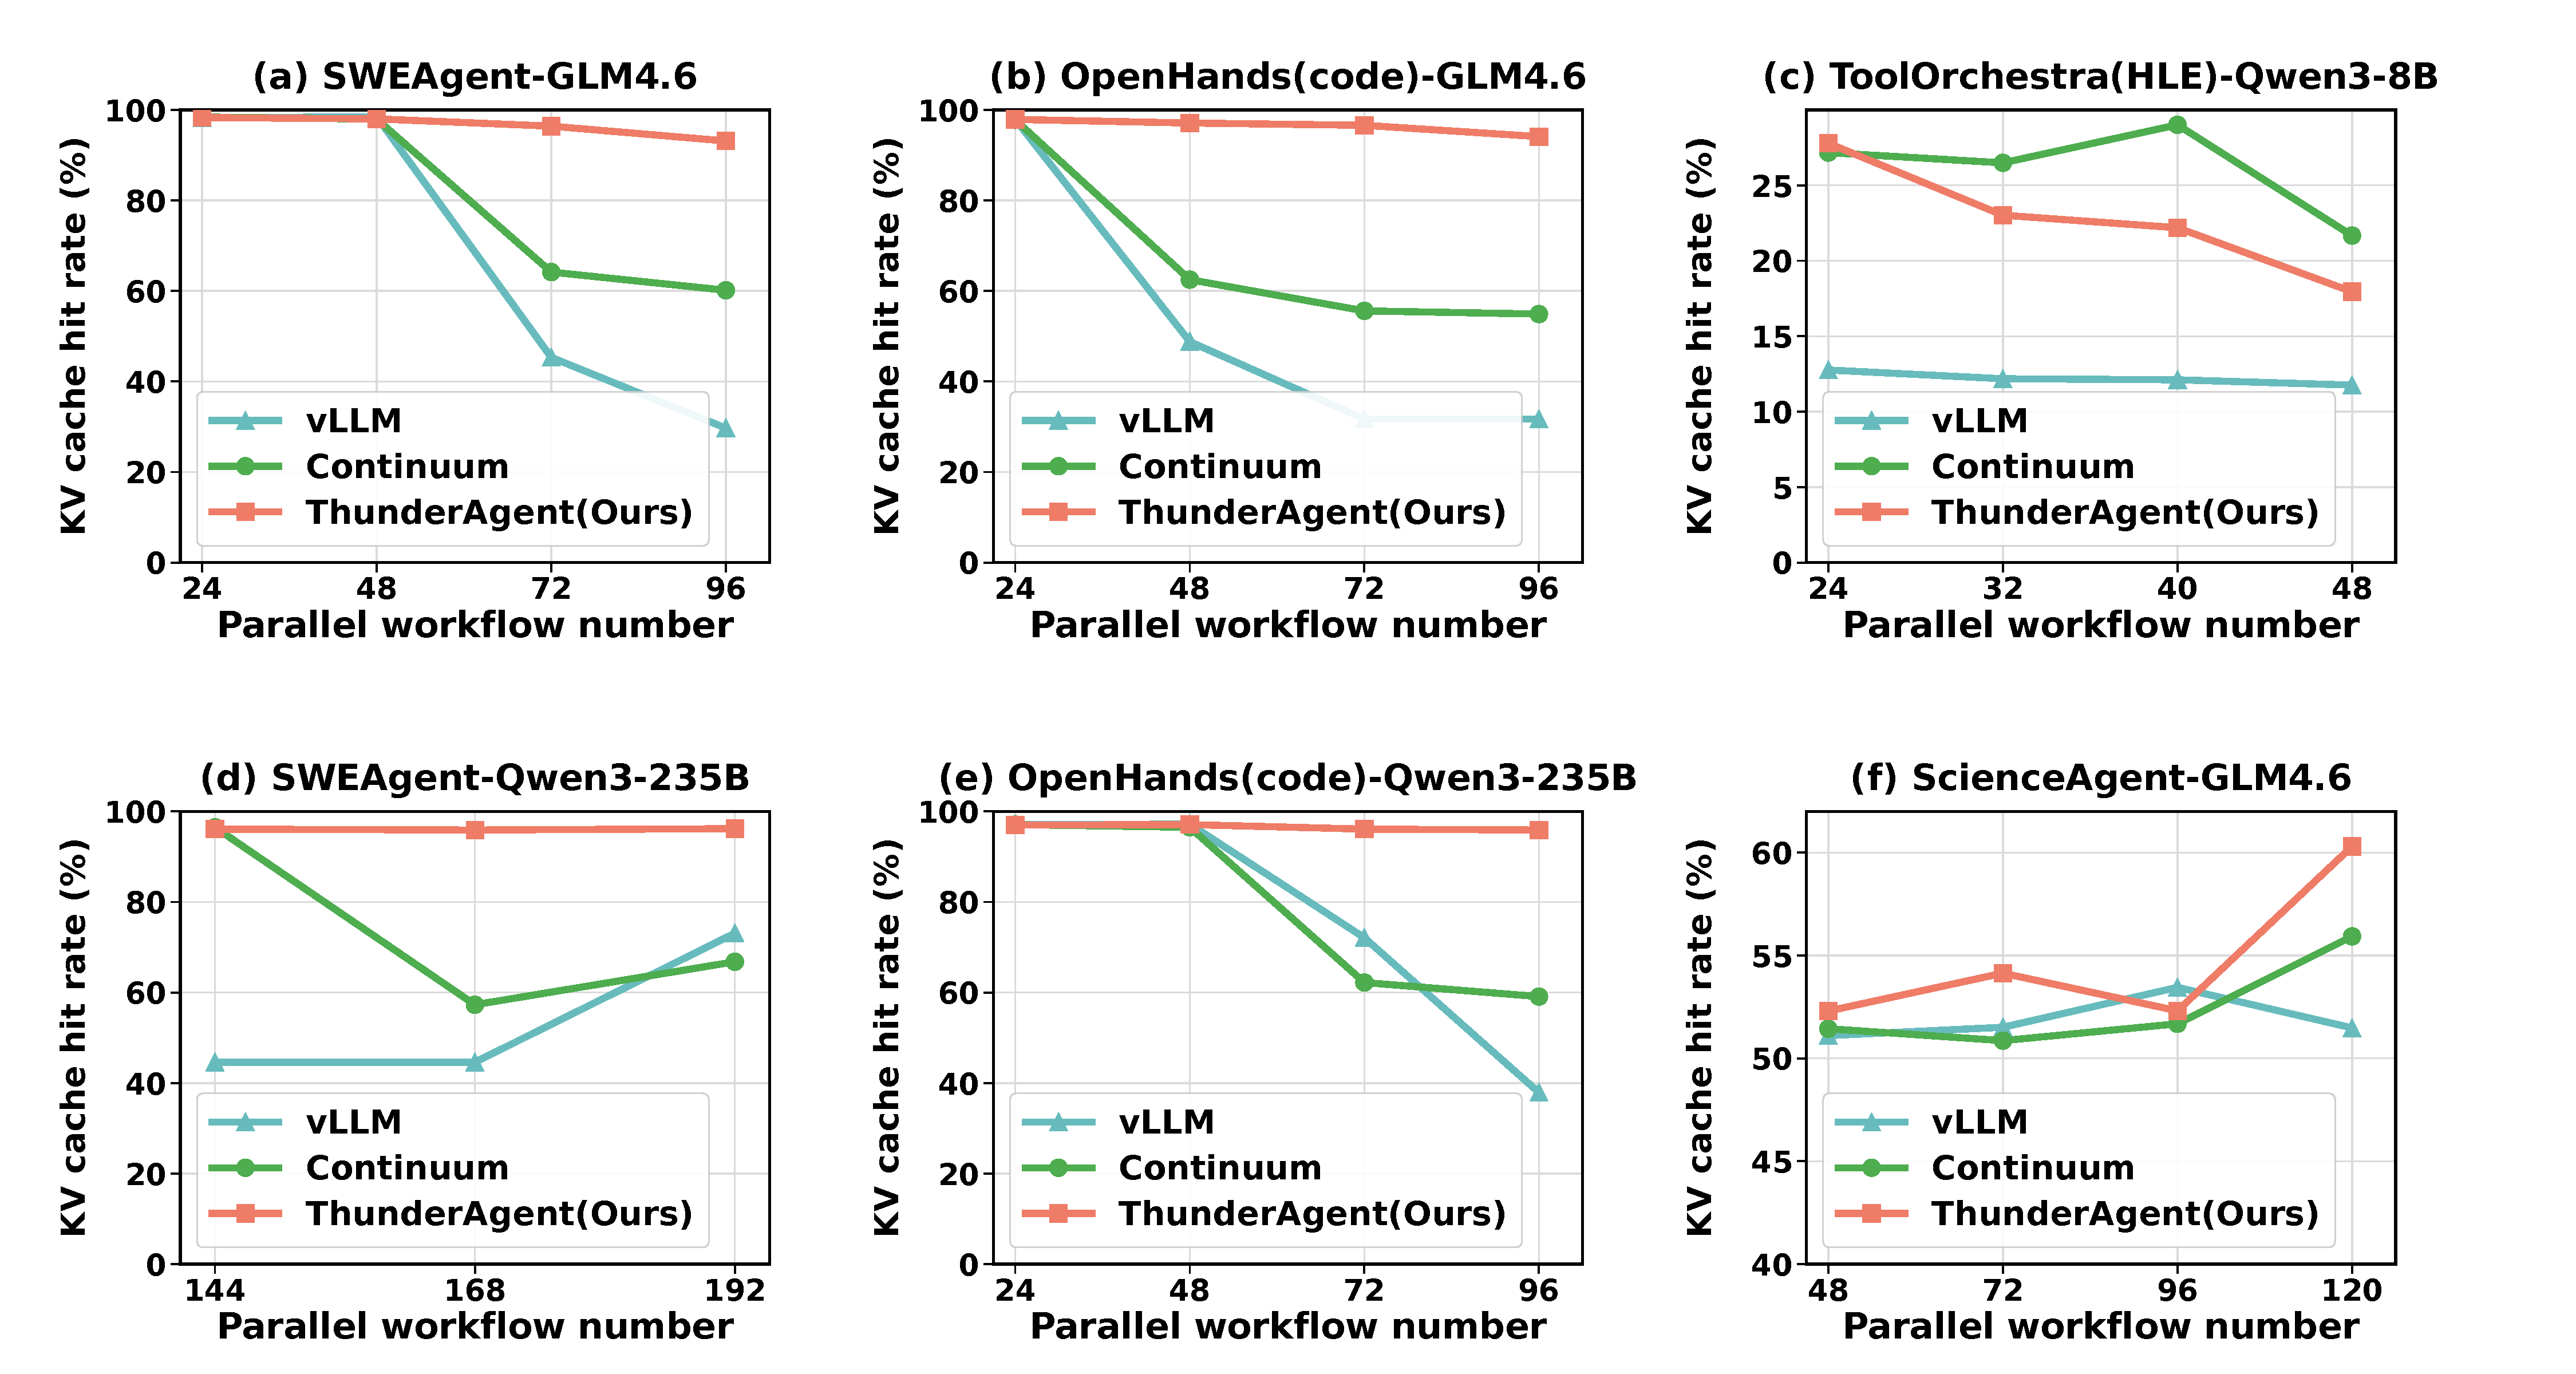
\includegraphics[width=\textwidth]{Figures/appendix_figs/kv_all.pdf}
  \caption{\textbf{KV Cache Hit Rate Statistics.} \ouralg achieves near-optimal ($\approx$ 100) hit rate with predictable tool call time (a, b, d, e), while dynamically trading hit rate for less idle caching with stochastic tool execution time (c, f). It also achieves higher KV cache hit rate in comparison to vLLM and Continuum.}
  \vspace{-1em}\label{fig:kv_hit_rate_data_statistics}
\end{figure*}
% We illustrate the throughput performance of~\ouralg compared to vLLM and Continuum in~\autoref{fig:eval_infer_result}, and \autoref{fig:kv_hit_rate_data_statistics} shows KV-cache hit rate among these settings. At high concurrency levels (e.g., 96 parallel programs), \ouralg demonstrates a substantial performance advantage. According to \autoref{fig:kv_hit_rate_data_statistics}, \ouralg reduces KV thrashing and maintains KV-cache hit rate by applying our scheduler discussed in \autoref{sec:scheduling_policy}. Even at lower concurrency (e.g., 24 parallel programs), \ouralg still achieves better throughput by reducing end-to-end latency and better tool resource management discussed in \autoref{sec:tool_resource}. Across different base models, agentic workflows, and datasets, \ouralg achieves a \textbf{1.48--3.58$\times$} speedup over vLLM and consistently outperforms Continuum by \textbf{1.17-3.31}$\times$.

\paragraph{High throughput under high concurrency.}
\autoref{fig:eval_infer_result} showcase that  \ouralg demonstrates superior throughput at high concurrency levels (e.g., 96 parallel programs), achieving a \textbf{1.48--3.58$\times$} speedup over vLLM and \textbf{1.17--3.31$\times$} speedup over Continuum across diverse base models and datasets.
This gain rises from our program-aware scheduler, which maintains a near-optimal KV cache hit rate ($\approx$100\% for Mini-SWE-Bench and OpenHands, see \autoref{fig:kv_hit_rate_data_statistics} a, b, d, e) and enables the asynchronous preparation of environments. In contrast, Continuum suffers from performance degradation under high concurrency. As shown in \autoref{fig:kv_hit_rate_data_statistics}, its KV cache hit rate drops significantly from $>$90\% to $\approx$60\%. This is because Continuum suffers from KV cache eviction among requests in different programs when no enough memory is available for ongoing requests' decoding. As a result, active programs compete for limited memory and trigger thrashing.

% \vspace{-1mm}
\paragraph{Robustness performance to high concurrency.}
\ouralg maintains maximum achievable throughput even as the parallel workflow number scales beyond the GPU memory limit. As showcased in \autoref{fig:eval_infer_result}, \ouralg ensures that throughput remains stable with the number of parallel workflows, whereas baseline systems suffer from severe throughput collapse once the workload exceeds memory limits. In practical agentic serving, statically determining the optimal parallel workflow number to maximize utilization with limited KV cache thrashing and caching cost is often infeasible due to the stochastic nature of agent environments and tool execution durations. \ouralg addresses this by automatically adapting to the maximum available capacity without manual tuning, a capability critical for robust real-world deployments.

\paragraph{Robustness across deterministic and stochastic tool executions.}
% \vspace{-1mm}
\ouralg outperforms baselines not only in workflows with deterministic tool patterns (\autoref{fig:eval_infer_result} a, b, d, e) but also under highly stochastic conditions (\autoref{fig:eval_infer_result} c, f).
This comes from our dynamic program-aware waiting queue policy. vLLM's request-aware scheduler typically lacks reserved memory for acting programs, forcing frequent re-computation. Conversely, Continuum statically reserves memory for all paused programs and mispredicts the tool execution time. These lead to expensive $\text{Cost}_{\text{recompute}}$ or $\text{Cost}_{\text{caching}}$ during long, unpredictable tool calls.
\ouralg balances them via a time-decay function $f(t)$, which prioritizes retaining KV cache for programs with short tool calls while preemptively pausing programs with long tool execution time to prevent memory waste.
As shown in \autoref{fig:kv_hit_rate_data_statistics} (right), although \ouralg exhibits a lower KV cache hit rate than Continuum in stochastic settings, it achieves higher throughput by ensuring active GPU utilization.

% \ouralg not only outperforms vLLM and Continuum under agentic workflows that have deterministic and sufficient tool calls(a,b,d,e in \autoref{fig:eval_infer_result}), but also under conditions where tool calls are stochastic(c,f in \autoref{fig:eval_infer_result}). This is because vLLM applies a request-aware scheduler that has zero KV-cache space for acting programs. While Continuum does give every acting program enough space to place its KV-cache, this might cause great memory underutilization for GPU. \ouralg dynamically trade-off cost of caching and recompute by applying a time decay function $f(t)$ that erases caching places when GPUs are underutilized, but keeps the KV-cache programs that have short tool calls. Shown in(c,f in \autoref{fig:kv_hit_rate_data_statistics}), \ouralg has a lower KV cache hit rate than Continuum but maintains higher throughput.

% \vspace{-1mm}
% Beyond the performance gains,~\ouralg maintains maximum achievable throughput when the program number increases after maximize hardware utilization. In practical agentic serving and rollout, determining the optimal parallel program number that maximizes hardware utilization without triggering KV-cache thrashing, is often infeasible due to the stochastic nature of agent environments and tool execution durations. Unlike baseline systems where exceeding this unknown threshold leads to throughput collapse, \ouralg ensures that throughput remains approximately \textbf{non-decreasing} as the number of parallel programs increases. This capability allows the system to automatically utilize the maximum available hardware capacity without manual tuning, which is critical for real-world deployments handling dynamic agentic workloads.

% In the distributed setting, we evaluated GLM-4.6 rollout on a two-node H100 cluster over a three-hour duration, measuring throughput in reasoning steps per minute. \ouralg demonstrates effective scalability with the number of nodes, achieving a \textbf{1.79--3.92$\times$} throughput increase. This improvement is driven by the system's ability to balance memory utilization across backends and mitigate thrashing, validating the effectiveness of \ouralg for memory-intensive, distributed agentic RL workloads.
\begin{figure}[t!]  % 使用 figure* 让图片跨越两栏
    \centering
    \begin{subfigure}{0.40\textwidth}
        \centering
        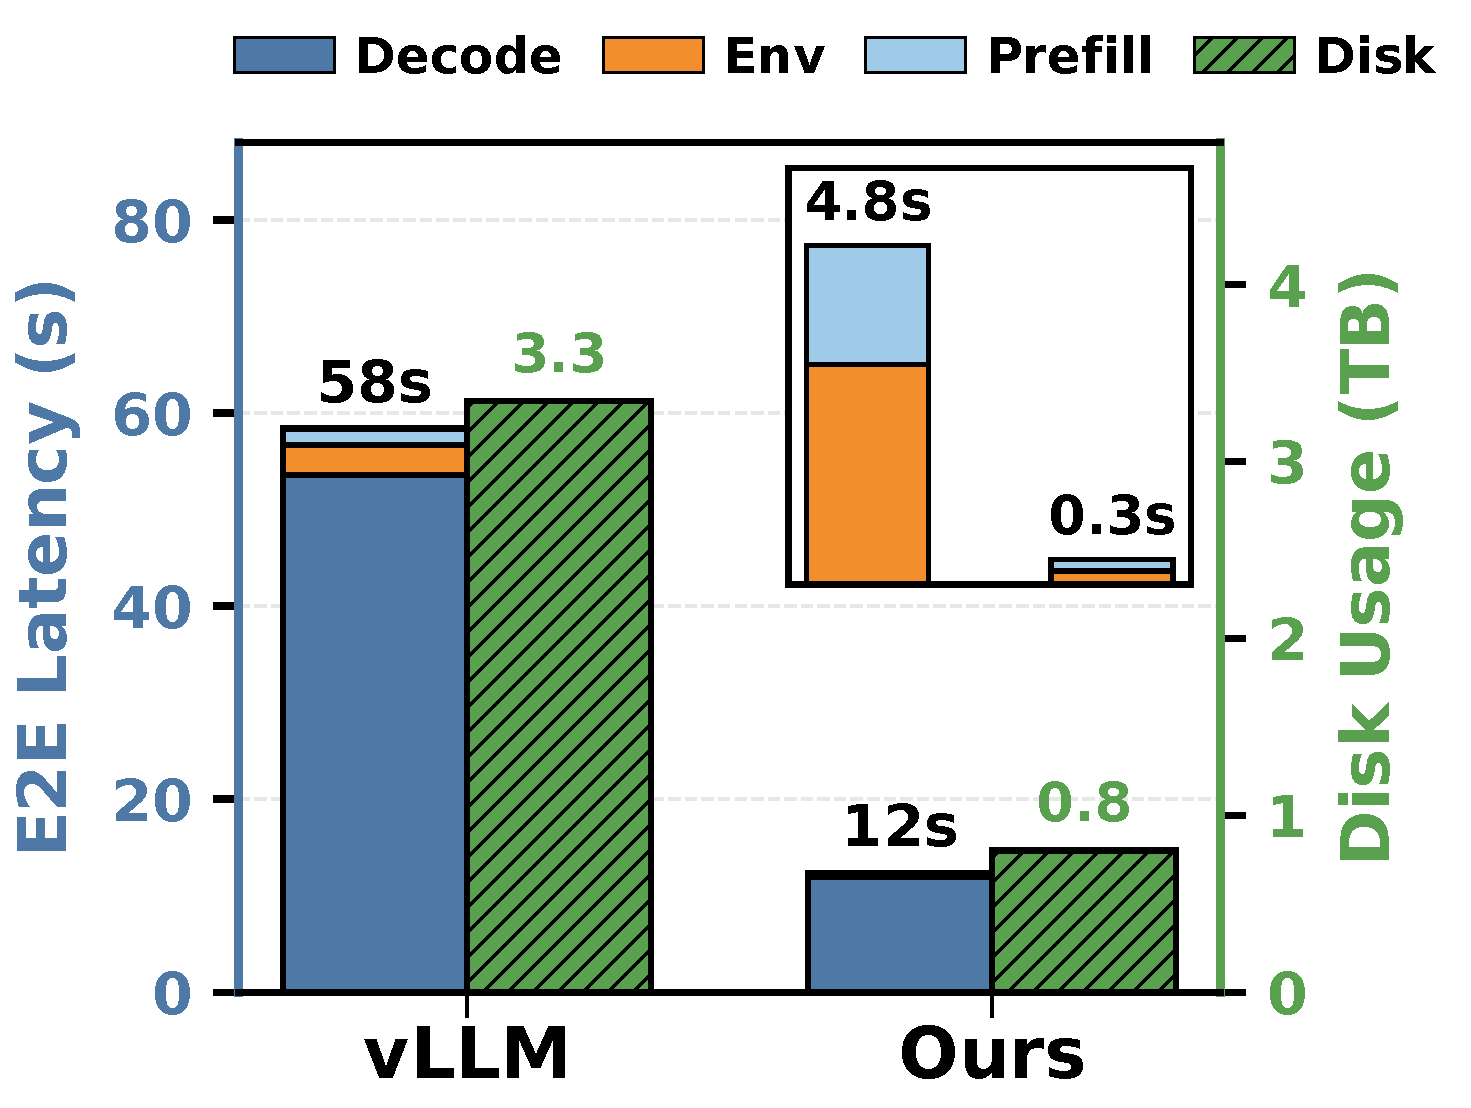
\includegraphics[width=0.99\textwidth]{Figures/e2e_breakdown.pdf}  % 替换为你的图片路径
        \caption{End-to-End Latency Breakdown}
        \label{fig:breakdown}
    \end{subfigure}
    \begin{subfigure}{0.33\textwidth}
        \centering
        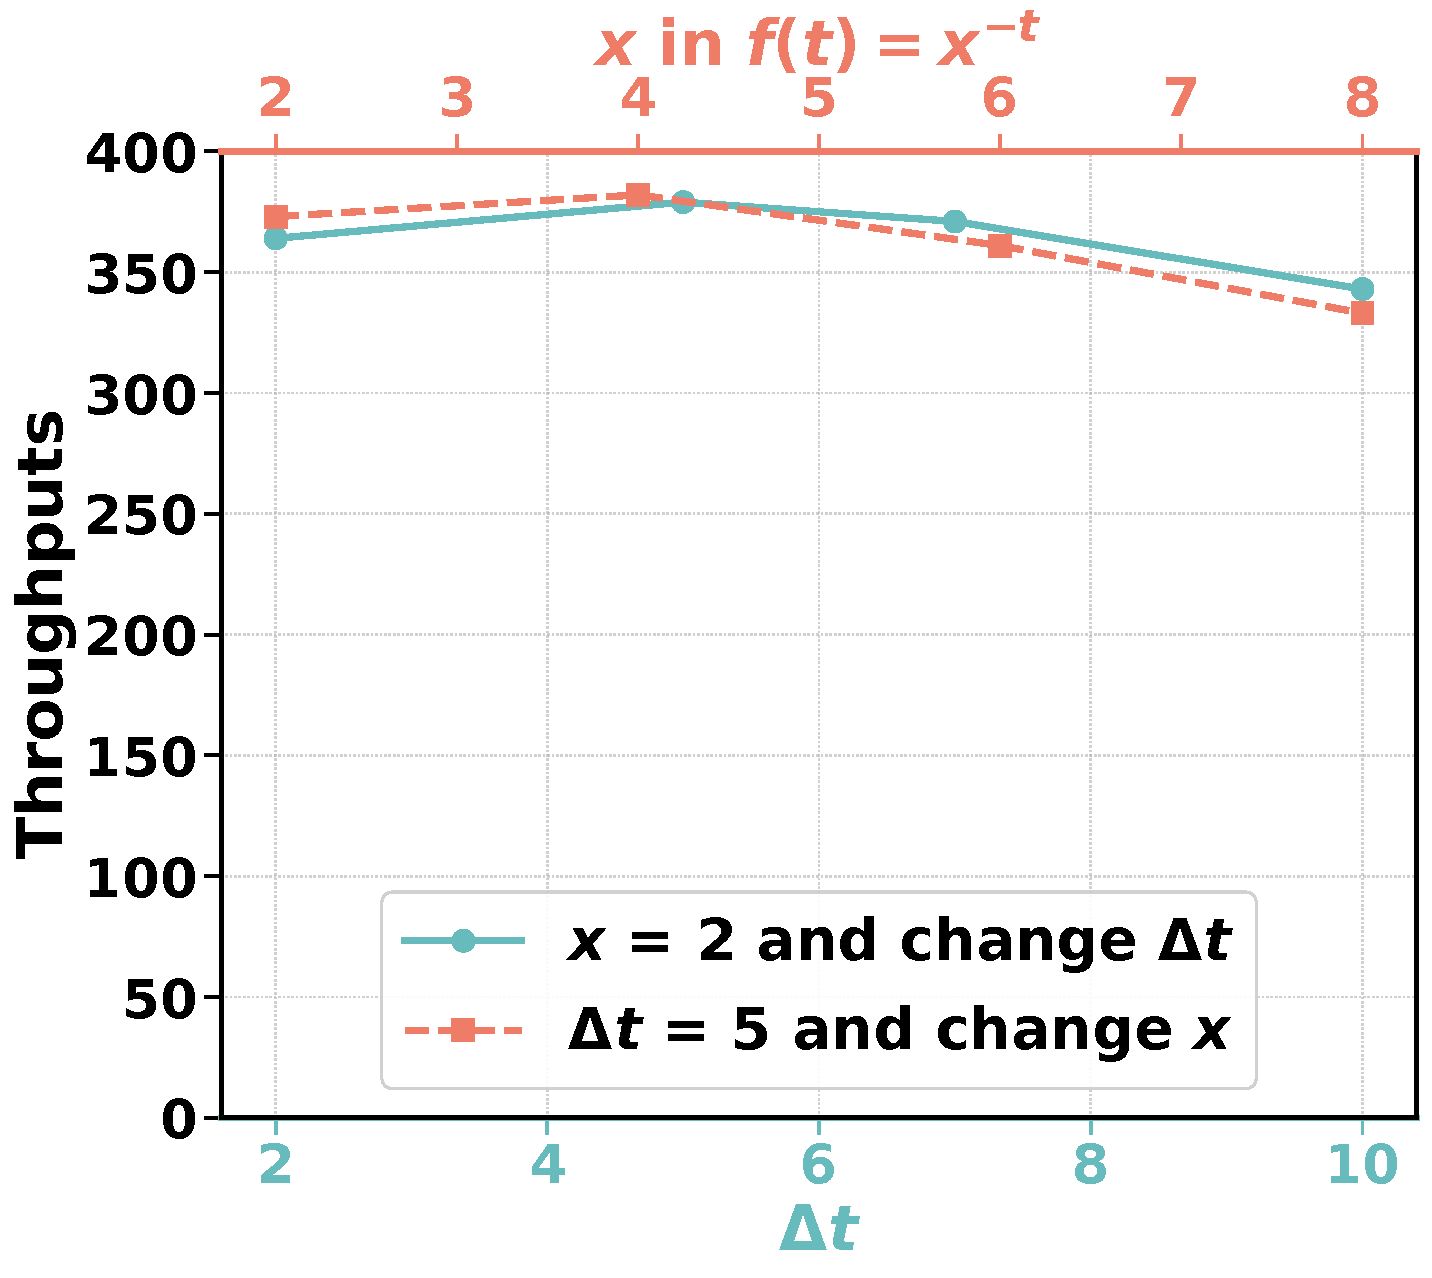
\includegraphics[width=0.99\textwidth]{Figures/parameter_ablation.pdf}  % 替换为你的图片路径
        \caption{Ablation of $\Delta t$ and f(t)}
        \label{fig:parameter_ablation}
    \end{subfigure}
    \caption{Ablation study of end-to-end latency breakdown and parameter sensitivity of \ouralg.}
    \label{fig:3}
    \vspace{-2mm}
\end{figure}


\vspace{-3mm}
\subsection{Rollout Evaluation Results}

% 紧凑版表格
\begin{wraptable}{r}{ 0.65\columnwidth}
\vspace{-1.1em}
\centering
\caption{\small \ouralg GLM-4.6 rollout ($N=144$) on 2$\times$H100 nodes.}
\vspace{-0.3em}
\label{tab:blocksize_ablation}
\resizebox{\linewidth}{!}{\setlength{\tabcolsep}{3mm}{
\begin{tabular}{llr}
\toprule
Workflow & Serving System & Throughput \\
\midrule
mini-SWEAgent & vLLM + Gateway & 375.4 \\
mini-SWEAgent & \ouralg & 671.8 (\textbf{1.79$\times$}) \\
OpenHands & vLLM + Gateway & 69.1 \\
OpenHands & \ouralg & 270.8 (\textbf{3.92$\times$}) \\
\bottomrule
\end{tabular}}}
\end{wraptable}

We evaluate RL rollout using GLM-4.6 on a two-node H100 cluster (3-hour duration). \autoref{tab:blocksize_ablation} shows that \ouralg can maintain effective scalability, achieving a \textbf{1.79--3.92$\times$} throughput increase over the vLLM $+$ Gateway baseline, making it highly efficient for memory-intensive distributed RL workloads.
% 删掉了 "This improvement is driven by..." 整句

\vspace{-2mm}
\subsection{Ablation Study}\label{app:ablation_study}
\paragraph{End-to-end latency breakdown.}
\autoref{fig:breakdown} decomposes the average end-to-end latency for OpenHands rollouts. The throughput gain stems primarily from reductions in \textbf{prefill and decode latency}. Moreover, the tool resource management policy (\autoref{sec:tool_resource}) contributes approximately \textbf{10\%} to the latency improvement while providing \textbf{4.2$\times$} disk memory savings. Per-step end-to-end latency are further discussed in \autoref{app:e2e}.
% 删掉了 "by reducing KV-cache thrashing..." 重复解释
% \begin{figure}[t!]  % 使用 figure* 让图片跨越两栏
%     \centering
%     \begin{subfigure}{0.40\textwidth}
%         \centering
%         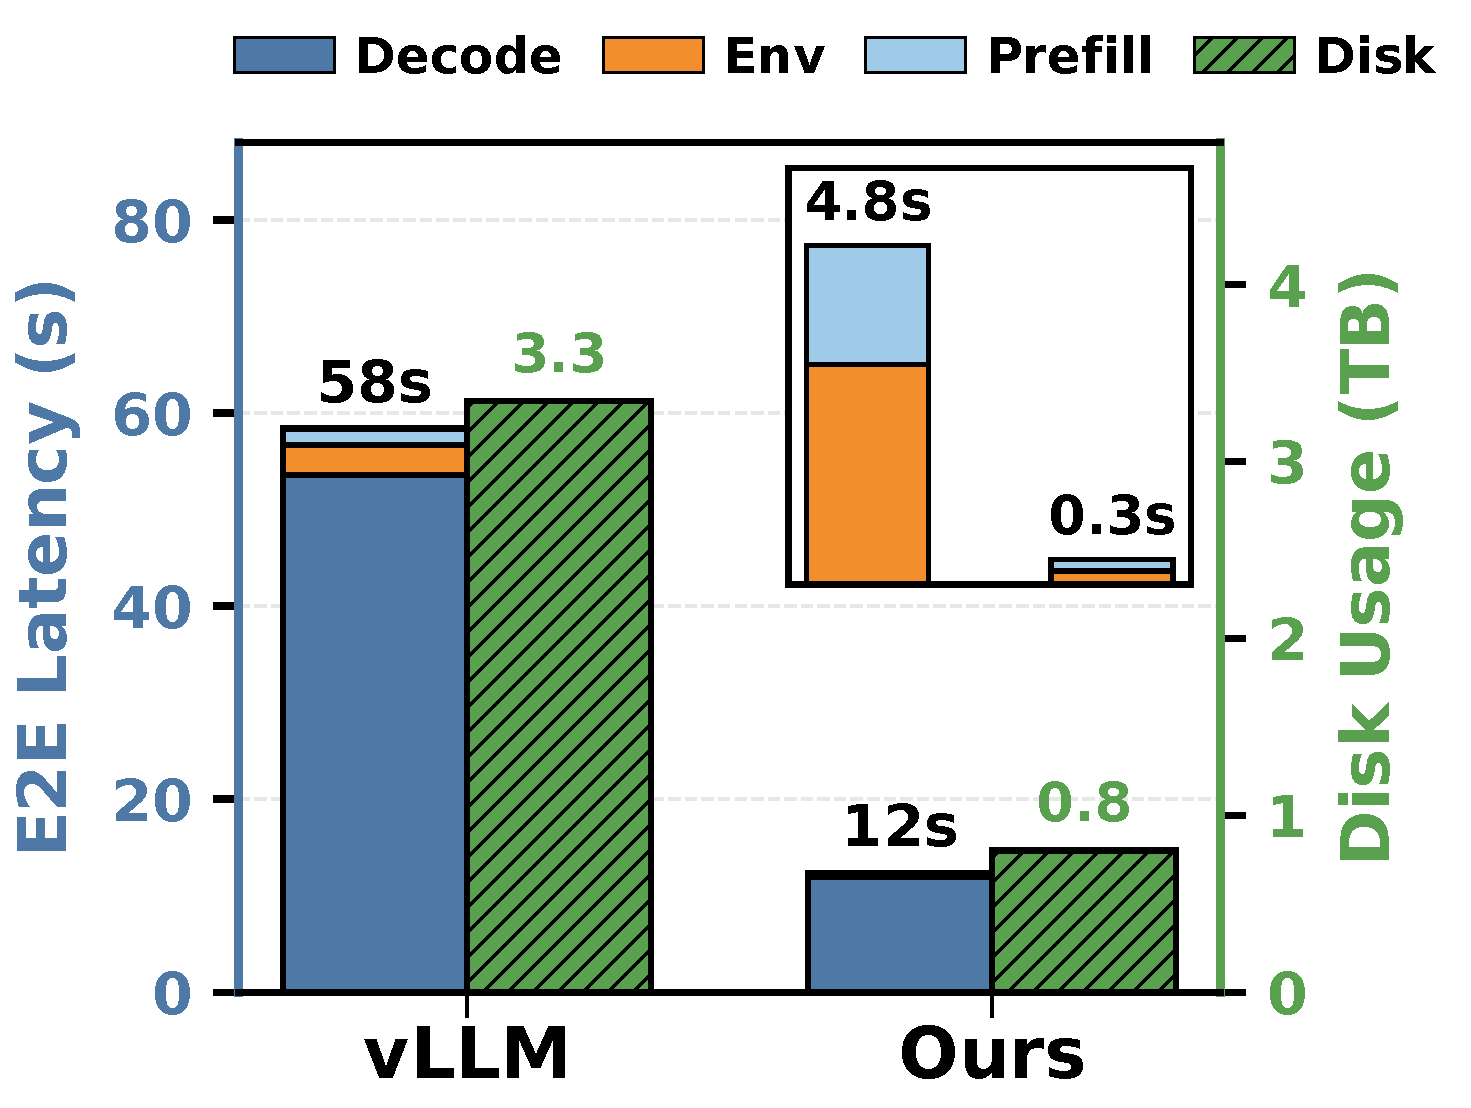
\includegraphics[width=0.99\textwidth]{Figures/e2e_breakdown.pdf}  % 替换为你的图片路径
%         \caption{End-to-end Latency}
%         \label{fig:breakdown}
%     \end{subfigure}
%     \begin{subfigure}{0.33\textwidth}
%         \centering
%         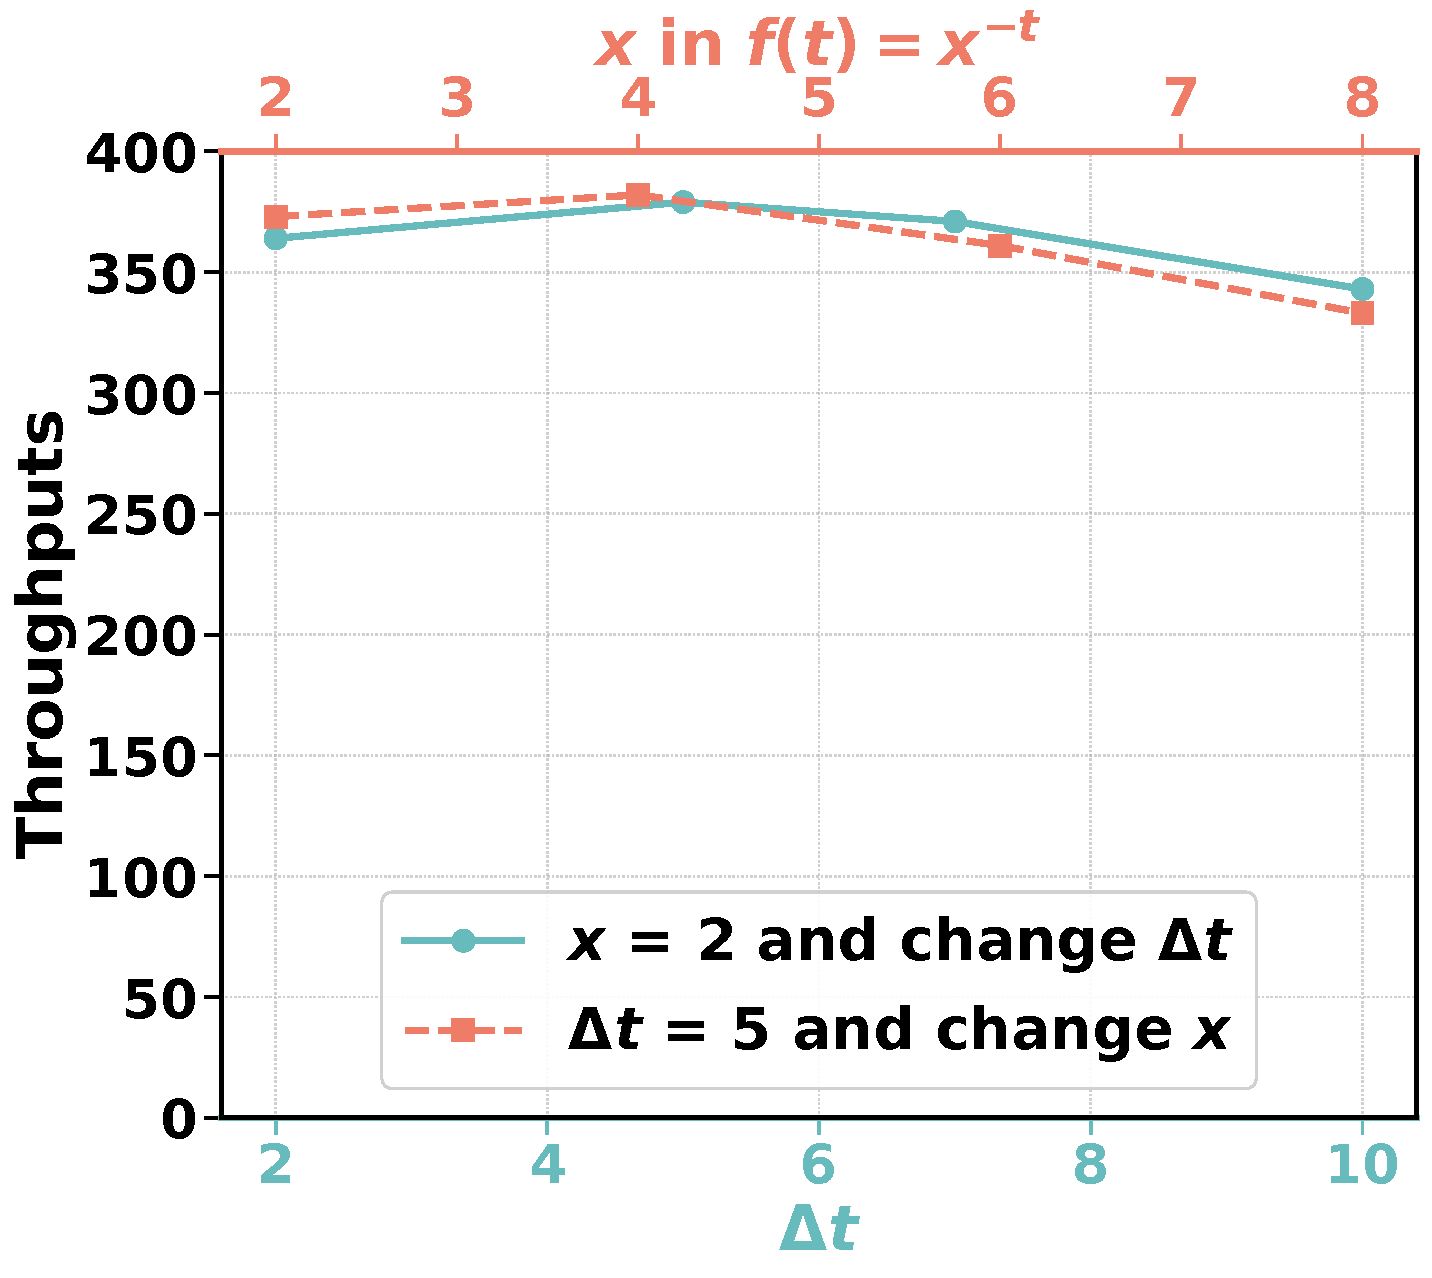
\includegraphics[width=0.99\textwidth]{Figures/parameter_ablation.pdf}  % 替换为你的图片路径
%         \caption{Ablation of $\Delta t$ and f(t)}
%         \label{fig:parameter_ablation}
%     \end{subfigure}
%     \caption{Ablation study of agentic RL rollout and parameter sensitivity of \ouralg.}
%     \label{fig:3}
% \end{figure}

\paragraph{Ablation on $\Delta t$ and f(t).} We study the sensitivity of detecting period $\Delta t$ and decaying function $f(t) = x^{-t}$. \autoref{fig:parameter_ablation}
 shows \ouralg offline serving mini-SWEAgent with GLM4.6 as base model on a single H100 node. We observe that \ouralg maintains high throughput under different parameter settings, demonstrating the robustness of our method. Further increasing $\Delta t$ might decrease the KV cache hit rate and thereby reduce throughput because thrashing might occur in the middle of detecting. Also, increasing $x$ in $f(t)$ allows more aggressive eviction of acting programs, which trade recomputation costs to reduce caching costs. This reduces throughput as acting programs
with short tool execution time are prematurely evicted.% \textbf{Ablation study on KV cache offloading.}
% We investigated KV cache offloading via LMcache as a potential remedy for capacity constraints. While offloading theoretically extends effective memory space by utilizing CPU or disk storage, our implementation with vLLM+LMcache reveals a critical bottleneck: the PCIe bandwidth is insufficient to sustain the high-frequency context switching and large-volume data transfers inherent to agentic workloads. As shown in \autoref{fig:kv_offload}, when serving GLM-4.6 with mini-SWEAgent, the latency penalty from frequent swap-in/swap-out operations negates the capacity benefits, resulting in severe throughput degradation under heavy loads.

% \textbf{Ablation study on Prefill-Decode (PD) disaggregation.}
% We also explored PD disaggregation, a standard optimization for chatbot serving designed to isolate the decoding phase from prefill interference. However, for agentic workloads which are characterized by continuous context growth, we observe that PD disaggregation \textbf{\textit{exacerbates}} thrashing. By physically partitioning the cluster into prefill-only and decode-only nodes, the effective HBM pool available for handling prefill is significantly smaller than in a unified architecture. This memory fragmentation causes the system to hit capacity limits and trigger thrashing at much lower concurrency levels, as shown in \autoref{fig:pd disaggregation}. \textbf{These results demonstrate that generic architectural optimizations cannot substitute for a program-centric scheduler that actively manages the working set.}
